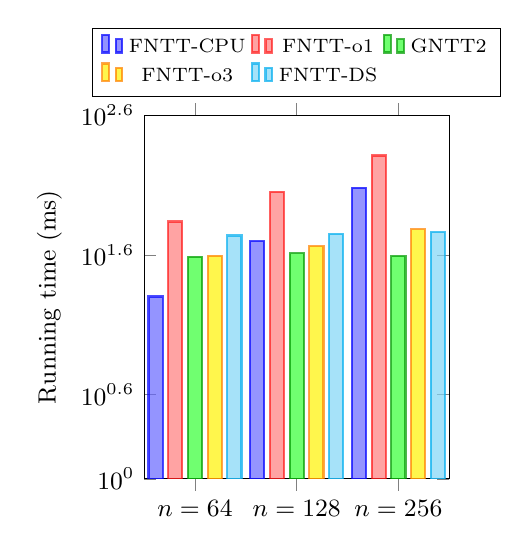
\begin{tikzpicture}
    \begin{axis}[
        ybar, 
        symbolic x coords={$n=64$, $n=128$, $n=256$},  ymode=log, 
        xtick=data,  
        xticklabel style={font=\small},
        yticklabel style={font=\small},
        ylabel={\small Running time (ms)},    
        width=0.45\linewidth,
        height=6.2cm,
        bar width=0.18cm,  
        enlarge x limits=0.25,  
        ymin=1,  
        ymax=400,
        ytick={1, 4, 40, 400}, 
        ylabel near ticks,
        legend style={
            at={(0.5,1.05)}, 
            anchor=south,    
            legend columns=3, 
            draw=black,      
            fill=white,    
            font=\scriptsize,
            legend image post style={scale=0.8} 
        },
    ]

    \addplot[fill=blue!60,draw=blue,thick,opacity=0.7]
     coordinates {($n=64$, 20.19) ($n=128$, 50.199) ($n=256$, 121.189)};  

    \addplot[fill=red!60,draw=red,thick,opacity=0.6]
     coordinates {($n=64$, 69.46) ($n=128$, 113.481) ($n=256$, 206.315)};  

    \addplot[fill=green!80,draw=green!60!black,thick,opacity=0.7]
     coordinates {($n=64$, 38.882) ($n=128$, 41.145) ($n=256$, 39.375)};   

     \addplot[fill=yellow,draw=orange,thick,opacity=0.7]
    coordinates {($n=64$, 39.54) ($n=128$, 46.226) ($n=256$, 61.044)};

    \addplot[fill=cyan!50,draw=cyan,thick,opacity=0.7]
    coordinates {($n=64$, 55.137) ($n=128$, 56.628) ($n=256$, 58.39)};

    \legend{FNTT-CPU, FNTT-o1, GNTT2, FNTT-o3, FNTT-DS}
    \end{axis}
\end{tikzpicture}